\section{Purpose of the laboratory work}

\begin{itemize}
	\item Obtaining testing skills for the functionalities of a software; 
	
	\item Studying the structural method of testing a program;
	
	\item Get to know White box testing technique;
\end{itemize}

\section{Laboratory Work Requirements}
\begin{itemize}
	\item Draw the graph of the control flow of the program;
	
	\item Test the program according to the coverage criteria;
	
	\item Emphasize samples for which are obtained erroneous results for different coverage criteria;

	\item Comment the special cases and the tests;
	
	\item Use McCabe technique to test basic paths;
	
	\item Make conclusions and present a report;
\end{itemize}

\section{Intro to the technique}

White-box testing (also known as clear box testing, glass box testing, transparent box testing, and structural testing) is a method of software testing that tests internal structures or workings of an application, as opposed to its functionality (i.e. black-box testing). 

In white-box testing an internal perspective of the system, as well as programming skills, are used to design test cases. The tester chooses inputs to exercise paths through the code and determine the expected outputs.

White-box testing can be applied at the unit, integration and system levels of the software testing process. Although traditional testers tended to think of white-box testing as being done at the unit level, it is used for integration and system testing more frequently today.

\begin{center}
	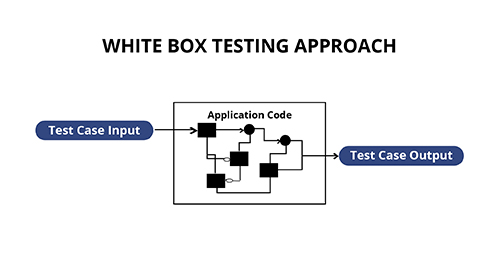
\includegraphics[scale=0.7]{images/Capture1}
\end{center}

\clearpage